\documentclass[12pt]{article}
%\usepackage[cp1251]{inputenc}
\usepackage[utf8]{inputenc}
\usepackage[bulgarian]{babel}
\usepackage{amssymb,amsmath,amsfonts,amstext,amscd,latexsym}
\usepackage{graphicx}
\usepackage{amsmath}
\usepackage[colorinlistoftodos]{todonotes}
\usepackage{systeme}
\usepackage[geometry]{ifsym}
\usepackage{listings}
\usepackage{float}
\usepackage{color}

\begin{document}
	\begin{titlepage}	
		\newcommand{\HRule}{\rule{\linewidth}{0.5mm}} % Defines a new command for the horizontal lines, change thickness here
		\begin{center}
		\textsc{\LARGE Софийски университет }\\[0.3cm]
		\textsc{\LARGE "Св. Климент Охридски" }\\[0.3cm]
		\textsc{\Large Факултет по математика и информатика }\\[0.2cm]
		%\fontsize{size}{baselineskip}
		
		{\fontsize{12}{18}\selectfont \bf МАШИННО САМООБУЧЕНИЕ}\vspace{15pt}\newline спец. Изкуствен интелект, I курс, зимен семестър \newline учебна година 2024/2025
		\vspace{30pt}
		
		
		
		
		
		\begin{minipage}{0.4\textwidth}
			\begin{flushleft}\large
				\emph{Изготвил:} \\
				Кристиян Симов \\ 
				фак. номер 4MI3400288
			\end{flushleft}
		\end{minipage}
		~
		%\begin{flushleft}
		\begin{minipage}{0.4\textwidth}
			\begin{flushright}
				\large
				\emph{Дата:}\\
				25. 10. 2024 г. % Попълнете датата на предаване
				\\София 
			\end{flushright}
		\end{minipage}\\[1cm]
		%\end{flushleft}
		\bigskip
		{\large \textbf{Домашна работа \textnumero 2}}\\[1cm] % Date, change the \today to a set date if you want to be precise
		%\includegraphics{rsz_sofia_university_logo.png}\\[1cm] 
		
\includegraphics{logo_su_no_text.png}\\[1cm]
		\vfill % Fill the rest of the page with whitespace
		\end{center}
	\end{titlepage}
	
	
	
	\tableofcontents
	
	
	
	\newpage
	
	\section{Решение на задача \textnumero 1}
	
	
	Нека имаме множество от обучаващи примери $S$ дефинирано чрез таблицата:
	\newline
	\begin{table}[h!]
	\centering
		\begin{tabular}{|c|c|c|c|}
			\hline
			Пример & Класификация & $A_{1}$ & $A_{2}$ \\ \hline				1      & +            & T       & T       \\ \hline
			2      & +            & T       & T       \\ \hline
			3      & -            & T       & F       \\ \hline
			4      & +            & F       & F       \\ \hline
			5      & -            & F       & T       \\ \hline
			6      & -            & F       & T       \\ \hline
		\end{tabular}
	\end{table}
	\newline
	
	\paragraph{a)}
	Формулата за изчисление на ентропия от информационната теория за произволно множество от примери $S$ с булеви стойности на целевата функция (+ или -) , показваща неговата еднородност, е:
	
	\begin{center}
		$Entropy(S) \equiv -p_{+}\log_2 p_{+} - p_{-}\log_2 p_{-}$,
	\end{center}
	където $p_{+}$ и $p_{-}$ са съответно отношенията на броя на положителните и отрицателните примери към броят всички примери.\newline\newline
	Прилагаме я към конкретното множество S и последователно получаваме:

	\begin{center}
	$Entropy([3_{+}, 3_{-}]) = -\frac{3}{6}\log_2 \frac{3}{6} - \frac{3}{6}\log_2 \frac{3}{6} = -\frac{1}{2}\log_2 \frac{1}{2} - \frac{1}{2}\log_2 \frac{1}{2} =\newline\newline= -\frac{1}{2}(-1) - \frac{1}{2}(-1) = \frac{1}{2} + \frac{1}{2} = 1$
	\end{center}

	Очаквано, получихме ентропия равна на 1, тъй като броят на положителните и отрицателните примери е еднакъв (в случая равен на 3).\newline
	\newpage
	\paragraph{b)}
	Формулата за изчисление информационната печалба на атрибут $A$ по отношение на произволно множество от примери $S$ е:
	
	\begin{center}
		$Gain(S, A) \equiv Entropy(S) - \displaystyle\sum_{v \in Values(A)} \frac{|S_{v}|}{|S|}Entropy(S_{v})$,
	\end{center}
	където $Values(A)$ е множеството от възможни стойности на атрибута $A$, а множеството $S_{v} = \{ s \in S | A(s) = v \}$.\newline\newline
	Прилагаме я към атрибута $A_{2}$ по отношение на конкретното множество S и последователно получаваме:
	
	\begin{equation*}
		\begin{split}
			Gain(S, A_{2}) & = Entropy(S) - \displaystyle\sum_{v \in Values(A_{2})} \frac{|S_{v}|}{|S|}Entropy(S_{v}) \\
			& = 1 - \displaystyle\sum_{v \in \{T, F\}} \frac{|S_{v}|}{6}Entropy(S_{v}) \\
			& = 1 - \frac{|S_{T}|}{6}Entropy(S_{T}) - \frac{|S_{F}|}{6}Entropy(S_{F}) \\
			& = 1 - \frac{4}{6}Entropy([2_{+}, 2_{-}]) - \frac{2}{6}Entropy([1_{+}, 1_{-}]) \\
			& = 1 - (\frac{4}{6})1 - (\frac{2}{6})1 \\
			& = 1 - 1 \\
			& = 0
		\end{split}
	\end{equation*}

	Очаквано, получихме печалба равна на 0, тъй като броят на положителните и отрицателните примери е еднакъв в подмножествата $S_{T}$ и $S_{F}$.\newline
	\newpage
	
	\section{Решение на задача \textnumero 2}
	\paragraph{a)}
	
	Нека имаме множество от обучаващи примери $S$ дефинирано чрез таблицата:
	\newline
	\begin{table}[!h]
	\centering
		\begin{tabular}{|c|c|c|c|c|c|c|c|}
			\hline
			\textit{Пример} & \textit{Небе} & \textit{Въздух} & \textit{Влажност} & \textit{Вятър} & \textit{Вода} & \textit{Прогноза} & \textit{Харесва} \\ \hline
			1               & Слънце        & Топъл           & Нормална          & Силен          & Топла         & Същото            & \textbf{да}      \\ \hline
			2               & Слънце        & Топъл           & Висока            & Силен          & Топла         & Същото            & \textbf{да}      \\ \hline
			3               & Дъжд          & Студен          & Висока            & Силен          & Топла         & Промяна           & \textbf{не}      \\ \hline
			4               & Слънце        & Топъл           & Висока            & Силен          & Студена       & Промяна           & \textbf{да}      \\ \hline
		\end{tabular}
	\end{table}
	\newline\newline
	Тогава алгоритъмът ID3 ще премине през рекурсивните извиквания:\newline
	
	\paragraph{0)} $S = \{x_{1}, x_{2}, x_{3}, x_{4}\}, A = \{A_{\textnormal{Небе}},  A_{\textnormal{Въздух}}, A_{\textnormal{Влажност}}, A_{\textnormal{Вятър}}, A_{\textnormal{Вода}}, A_{\textnormal{Прогноза}}\}$
	\subparagraph{}
	$Entropy(S) = Entropy([3_{\textbf{да}}, 1_{\textbf{не}}]) = -\frac{3}{4}\log_2 \frac{3}{4} - \frac{1}{4}\log_2 \frac{1}{4}  \approx 0.811 $
	\subparagraph{}
	\begin{equation*}
		\begin{split}
			Gain(A_{\textnormal{Небе}}, S) & = Entropy(S) - \frac{3}{4}Entropy([3_{\textbf{да}}, 0_{\textbf{не}}]) - \frac{1}{4}Entropy([0_{\textbf{да}}, 1_{\textbf{не}}])\\
			& \approx 0.811 - \frac{3}{4}0 - \frac{1}{4}0 \approx 0.811 - 0 - 0 \approx 0.811 \leftarrow best (max)
		\end{split}
	\end{equation*}
	\newline Тъй като при атрибут $A_{\textnormal{Небе}}$ достигнахме максималната стойност на функцията $Gain(A, S)$ е излишно да пресмятаме останалите печалби.
	\newline
	\begin{figure}[H]
		\centering
		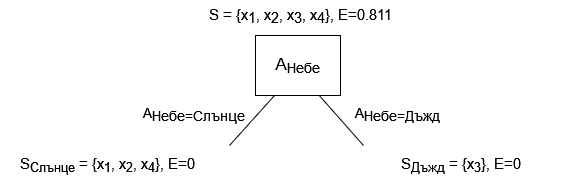
\includegraphics[width=80mm]{2a-0.png} 
		\caption{Построяваме клон за $A_{\textnormal{Небе}}=\textnormal{Слънце}$ и $A_{\textnormal{Небе}}=\textnormal{Дъжд}$. Разделяме множеството $S$ на $S_{\text{Слънце}}=\{x_{1}, x_{2}, x_{4}\}$ и $S_{\text{Дъжд}}=\{x_{3}\}$ и извикваме ID3 върху всяко от тях, но с множество $A \setminus {A_{\textnormal{Небе}}}$.}
	\end{figure}
	\newpage
	
	\paragraph{1)}
	 $S_{\textnormal{Слънце}} = \{x_{1}, x_{2}, x_{4}\},  A = \{A_{\textnormal{Въздух}}, A_{\textnormal{Влажност}}, A_{\textnormal{Вятър}}, A_{\textnormal{Вода}}, A_{\textnormal{Прогноза}}\}$
	\subparagraph{}
	$Entropy(S_{\textnormal{Слънце}}) = Entropy([3_{\textbf{да}}, 0_{\textbf{не}}]) = 0$
	\subparagraph{}
	Множеството $S_{\textnormal{Слънце}}$ е напълно еднородно - образуваме листо ``да''.
	\subparagraph{}
	Не се генерират повече рекурсивни извиквания на ID3.
	\paragraph{2)}
	$S_{\textnormal{Дъжд}} = \{x_{3}\},  A = \{A_{\textnormal{Въздух}}, A_{\textnormal{Влажност}}, A_{\textnormal{Вятър}}, A_{\textnormal{Вода}}, A_{\textnormal{Прогноза}}\}$
	\subparagraph{}
	$Entropy(S_{\textnormal{Дъжд}}) = Entropy([0_{\textbf{да}}, 1_{\textbf{не}}]) = 0$
	\subparagraph{}
	Множеството $S_{\textnormal{Дъжд}}$ е напълно еднородно - образуваме листо ``не''.
	\subparagraph{}
	Не се генерират повече рекурсивни извиквания на ID3.
	\newline\newline
	Край - дървото е обучено и след 1) и 2) изглежда така:
	\newline
		\begin{figure}[H]
		\centering
		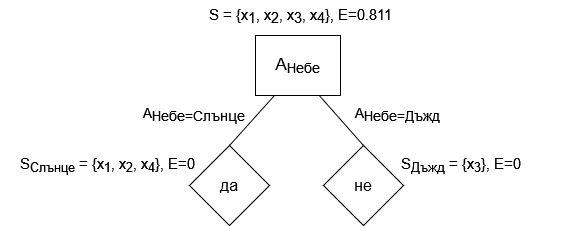
\includegraphics[width=100mm]{2a.png} 
		\caption{На изображението виждаме, че още след първото най-добро разделяне дървото е обучено успешно.}
	\end{figure}
	\newpage
	\paragraph{b)}
	
	Нека към предходната таблица за $S$ прибавим още един обучаващ пример:
	\newline
	\begin{table}[!h]
		\centering
		\begin{tabular}{|c|c|c|c|c|c|c|c|}
			\hline
			\textit{Пример} & \textit{Небе} & \textit{Въздух} & \textit{Влажност} & \textit{Вятър} & \textit{Вода} & \textit{Прогноза} & \textit{Харесва} \\ \hline
			1               & Слънце        & Топъл           & Нормална          & Силен          & Топла         & Същото            & \textbf{да}      \\ \hline
			2               & Слънце        & Топъл           & Висока            & Силен          & Топла         & Същото            & \textbf{да}      \\ \hline
			3               & Дъжд          & Студен          & Висока            & Силен          & Топла         & Промяна           & \textbf{не}      \\ \hline
			4               & Слънце        & Топъл           & Висока            & Силен          & Студена       & Промяна           & \textbf{да}      \\ \hline
			5               & Слънце        & Топъл           & Нормална            & Слаб          & Топла       & Същото           & \textbf{не}      \\ \hline
		\end{tabular}
	\end{table}
	\newline\newline
	Тогава алгоритъмът ID3 ще премине през рекурсивните извиквания:\newline
	
	
	\paragraph{0)} $S = \{x_{1}, x_{2}, x_{3}, x_{4}, x_{5}\},  A = \{A_{\textnormal{Небе}},  A_{\textnormal{Въздух}}, A_{\textnormal{Влажност}}, A_{\textnormal{Вятър}}, A_{\textnormal{Вода}}, A_{\textnormal{Прогноза}}\}$
	\subparagraph{}
	$Entropy(S) = Entropy([3_{\textbf{да}}, 2_{\textbf{не}}]) = -\frac{3}{5}\log_2 \frac{3}{5} - \frac{2}{5}\log_2 \frac{2}{5}  \approx 0.970 $
	\subparagraph{}
	\begin{equation*}
		\begin{split}
			Gain(A_{\textnormal{Небе}}, S) & \approx 0.970 - (\frac{1}{5}Entropy([0_{\textbf{да}}, 1_{\textbf{не}}]) + \frac{4}{5}Entropy([3_{\textbf{да}}, 1_{\textbf{не}}]))\\
			& \approx 0.970 - \frac{1}{5}0 - \frac{4}{5}0.811 \approx 0.970 - 0.65 \approx 0.32
		\end{split}
	\end{equation*}
	\subparagraph{}
	\begin{equation*}
		\begin{split}
			Gain(A_{\textnormal{Въздух}}, S) = Gain(A_{\textnormal{Небе}}, S) \approx 0.32
		\end{split}
	\end{equation*}
	\subparagraph{}
	\begin{equation*}
		\begin{split}
			Gain(A_{\textnormal{Влажност}}, S) & \approx 0.970 - (\frac{2}{5}Entropy([1_{\textbf{да}}, 1_{\textbf{не}}]) + \frac{3}{5}Entropy([2_{\textbf{да}}, 1_{\textbf{не}}]))\\
			& \approx 0.970 - \frac{2}{5}1 - \frac{3}{5}0.918 \approx 0.970 - 0.55 \approx 0.42 \leftarrow best
		\end{split}
	\end{equation*}
	\subparagraph{}
	\begin{equation*}
		\begin{split}
			Gain(A_{\textnormal{Вятър}}, S) = Gain(A_{\textnormal{Небе}}, S) \approx 0.32
		\end{split}
	\end{equation*}
	\subparagraph{}
	\begin{equation*}
		\begin{split}
			Gain(A_{\textnormal{Вода}}, S) & \approx 0.970 - (\frac{1}{5}Entropy([1_{\textbf{да}}, 0_{\textbf{не}}]) + \frac{4}{5}Entropy([2_{\textbf{да}}, 2_{\textbf{не}}]))\\
			& \approx 0.970 - \frac{1}{5}0 - \frac{4}{5}1 \approx 0.970 - 0.8 \approx 0.17
		\end{split}
	\end{equation*}
	\subparagraph{}
	\begin{equation*}
		\begin{split}
			Gain(A_{\textnormal{Прогноза}}, S) = Gain(A_{\textnormal{Влажност}}, S) \approx 0.42
		\end{split}
	\end{equation*}
	Тъй като $Gain(A_{\textnormal{Прогноза}}, S) \leq Gain(A_{\textnormal{Влажност}}, S) = 0.42$, то 0.42 е максималната печалба, достигната първо при атрибута $A_{\textnormal{Влажност}}.$
	\newline
	\begin{figure}[H]
		\centering
		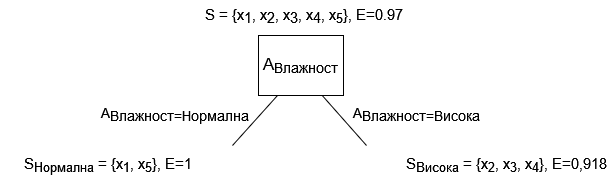
\includegraphics[width=120mm]{2b-0.png} 
		\caption{Построяваме клон за $A_{\textnormal{Влажност}}=\textnormal{Нормална}$ и $A_{\textnormal{Влажност}}=\textnormal{Висока}$. Разделяме множеството $S$ на $S_{\text{Нормална}}=\{x_{1}, x_{5}\}$ и $S_{\text{Висока}}=\{x_{2}, x_{3}, x_{4}\}$ и извикваме ID3 върху всяко от тях, но с множество $A \setminus {A_{\textnormal{Влажност}}}$.}
	\end{figure}
	\newpage
	
	\paragraph{1)}
	$S_{\textnormal{Нормална}} = \{x_{1}, x_{5}\},  A = \{A_{\textnormal{Небе}},  A_{\textnormal{Въздух}}, A_{\textnormal{Вятър}}, A_{\textnormal{Вода}}, A_{\textnormal{Прогноза}}\}$
	\subparagraph{}
	$Entropy(S_{\textnormal{Нормална}}) = Entropy([1_{\textbf{да}}, 1_{\textbf{не}}]) = -\frac{1}{2}\log_2 \frac{1}{2}  - \frac{1}{2}\log_2 \frac{1}{2} = 1$
	\subparagraph{}
	\begin{equation*}
		\begin{split}
			Gain(A_{\textnormal{Небе}}, S_{\textnormal{Нормална}}) & = Gain(A_{\textnormal{Въздух}}, S_{\textnormal{Нормална}}) \\
			& = Gain(A_{\textnormal{Вода}}, S_{\textnormal{Нормална}}) \\
			& = Gain(A_{\textnormal{Прогноза}}, S_{\textnormal{Нормална}}) \\
			& = 1 - Entropy([1_{\textbf{да}}, 1_{\textbf{не}}]) \\
			& = 1 - 1 = 0
		\end{split}
	\end{equation*}
	\subparagraph{}
	\begin{equation*}
		\begin{split}
			Gain(A_{\textnormal{Вятър}}, S_{\textnormal{Нормална}}) & = 1 - Entropy([1_{\textbf{да}}, 0_{\textbf{не}}]) - Entropy([0_{\textbf{да}}, 1_{\textbf{не}}]) \\ 
			& = 1 - 0 - 0 = 1 \leftarrow best
		\end{split}
	\end{equation*}
	Тъй като $Gain(A_{\textnormal{Вятър}}, S_{\textnormal{Нормална}}) = 1$, то това е максималната печалба, достигната при атрибута $A_{\textnormal{Вятър}}.$
	\newline
	\begin{figure}[H]
		\centering
		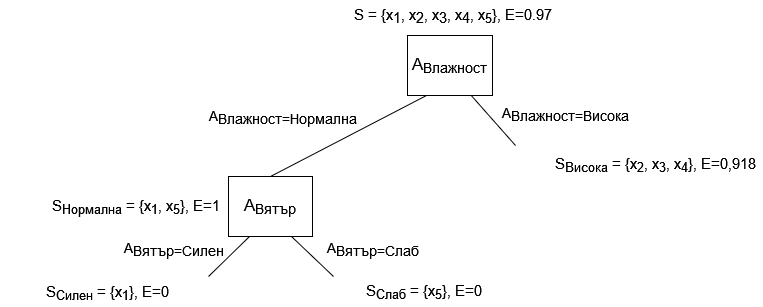
\includegraphics[width=150mm]{2b-1.png} 
		\caption{Построяваме клон за $A_{\textnormal{Вятър}}=\textnormal{Силен}$ и $A_{\textnormal{Вятър}}=\textnormal{Слаб}$. Разделяме множеството $S_{\textnormal{Нормална}}$ на $S_{\text{Силен}}=\{x_{1}\}$ и $S_{\text{Слаб}}=\{x_{5}\}$ и извикваме ID3 върху всяко от тях, но с множество $A \setminus {A_{\textnormal{Вятър}}}$.}
	\end{figure}
	\newpage
	\paragraph{2)}
	$S_{\text{Силен}}=\{x_{1}\}, A = \{A_{\textnormal{Небе}},  A_{\textnormal{Въздух}}, A_{\textnormal{Вода}}, A_{\textnormal{Прогноза}}\}$
	\subparagraph{}
	$Entropy(S_{\textnormal{Силен}}) = Entropy([1_{\textbf{да}}, 0_{\textbf{не}}]) = 0$
	\subparagraph{}
	Множеството $S_{\textnormal{Силен}}$ е напълно еднородно - образуваме листо ``да''.
	\subparagraph{}
	Не се генерират повече рекурсивни извиквания на ID3.
	\paragraph{3)}
	$S_{\textnormal{Слаб}} = \{x_{5}\},  A = \{A_{\textnormal{Небе}},  A_{\textnormal{Въздух}}, A_{\textnormal{Вода}}, A_{\textnormal{Прогноза}}\}$
	\subparagraph{}
	$Entropy(S_{\textnormal{Слаб}}) = Entropy([0_{\textbf{да}}, 1_{\textbf{не}}]) = 0$
	\subparagraph{}
	Множеството $S_{\textnormal{Слаб}}$ е напълно еднородно - образуваме листо ``не''.
	\subparagraph{}
	Не се генерират повече рекурсивни извиквания на ID3.
	\newline\newline
	След 2) и 3) дървото вече изглежда така:
	\newline
	\begin{figure}[H]
		\centering
		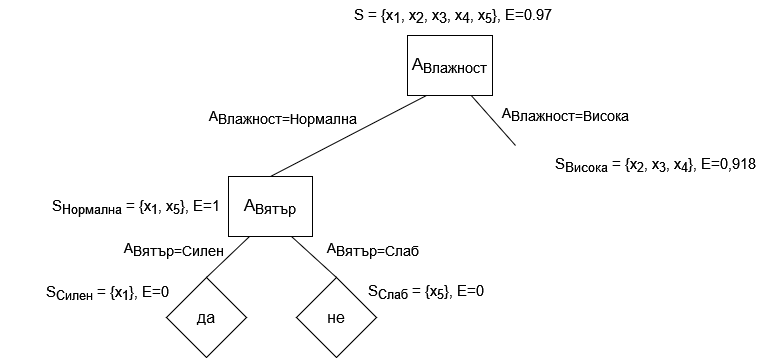
\includegraphics[width=150mm]{2b-2-3.png} 
		\caption{На изображението виждаме, че лявото поддърво е обучено успешно. Предстои рекурсията да се върне и обработи дясното поддърво.}
	\end{figure}
	\newpage
	
	\paragraph{4)}
	$S_{\textnormal{Висока}} = \{x_{2}, x_{3}, x_{4}\},  A = \{A_{\textnormal{Небе}},  A_{\textnormal{Въздух}},  A_{\textnormal{Вода}}, A_{\textnormal{Прогноза}}\}$
		\subparagraph{}
	$Entropy(S_{\textnormal{Висока}}) = Entropy([2_{\textbf{да}}, 1_{\textbf{не}}]) = -\frac{2}{3}\log_2 \frac{2}{3}  - \frac{1}{3}\log_2 \frac{1}{3} \approx 0.918$
	\subparagraph{}
	\begin{equation*}
		\begin{split}
			Gain(A_{\textnormal{Небе}}, S_{\textnormal{Висока}}) & \approx 0.918 - (\frac{2}{3}Entropy([2_{\textbf{да}}, 0_{\textbf{не}}]) + \frac{1}{3}Entropy([0_{\textbf{да}}, 1_{\textbf{не}}]))\\
			& \approx 0.918 - (\frac{2}{3}0 + \frac{1}{3}0) \\
			& \approx 0.918 - 0 \approx 0.918 \leftarrow best (max)
		\end{split}
	\end{equation*}
	Тъй като при атрибут $A_{\textnormal{Небе}}$ достигнахме максималната стойност на функцията $Gain(A, S_{\textnormal{Висока}})$ е излишно да пресмятаме останалите печалби.
	\newline
	\begin{figure}[H]
		\centering
		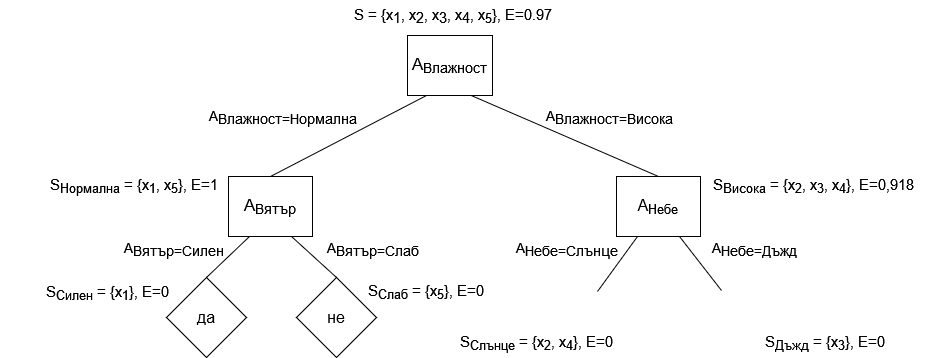
\includegraphics[width=150mm]{2b-4.png} 
		\caption{Построяваме клон за $A_{\textnormal{Небе}}=\textnormal{Слънце}$ и $A_{\textnormal{Небе}}=\textnormal{Дъжд}$. Разделяме множеството $S_{\textnormal{Висока}}$ на $S_{\text{Слънце}}=\{x_{2}, x_{4}\}$ и $S_{\text{Дъжд}}=\{x_{3}\}$ и извикваме ID3 върху всяко от тях, но с множество $A \setminus {A_{\textnormal{Небе}}}$.}
	\end{figure}
	\newpage
	
	\paragraph{5)}
	$S_{\text{Слънце}}=\{x_{2}, x_{4}\},  A = \{A_{\textnormal{Въздух}}, A_{\textnormal{Вятър}}, A_{\textnormal{Вода}}, A_{\textnormal{Прогноза}}\}$
	\subparagraph{}
	$Entropy(S_{\textnormal{Слънце}}) = Entropy([2_{\textbf{да}}, 0_{\textbf{не}}]) = 0$
	\subparagraph{}
	Множеството $S_{\textnormal{Слънце}}$ е напълно еднородно - образуваме листо ``да''.
	
	\paragraph{6)}
	$S_{\textnormal{Дъжд}} = \{x_{3}\},  A = \{A_{\textnormal{Въздух}}, A_{\textnormal{Вятър}}, A_{\textnormal{Вода}}, A_{\textnormal{Прогноза}}\}$
	\subparagraph{}
	$Entropy(S_{\textnormal{Дъжд}}) = Entropy([0_{\textbf{да}}, 1_{\textbf{не}}]) = 0$
	\subparagraph{}
	Множеството $S_{\textnormal{Дъжд}}$ е напълно еднородно - образуваме листо ``не''.
	\newline\newline
	Край - дървото е обучено и след 5) и 6) изглежда така:
	\newline
	\begin{figure}[H]
		\centering
		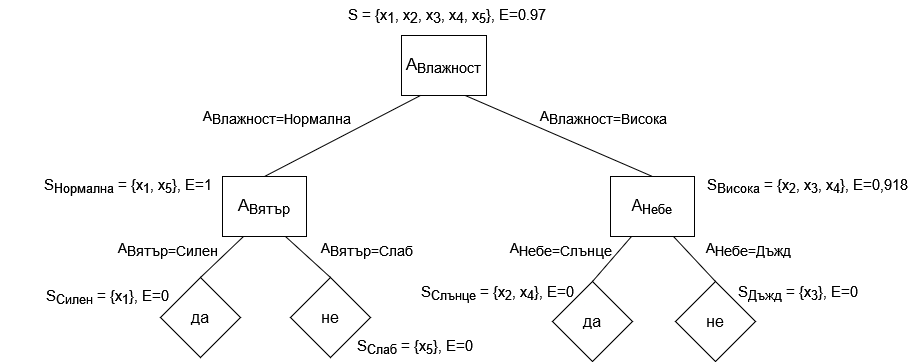
\includegraphics[width=150mm]{2b-5-6.png} 
		\caption{На изображението виждаме, че вече след първото най-добро разделяне се налага ID3 да избере още едно такова както за множеството в лявото поддърво, така и за това в дясното поддърво, след което дървото е обучено успешно.}
	\end{figure}
		
	\newpage
	
	\section{Решение на задача \textnumero 3}
	
	\paragraph{a)} $A \land \neg B$
		\begin{figure}[H]
			\centering
			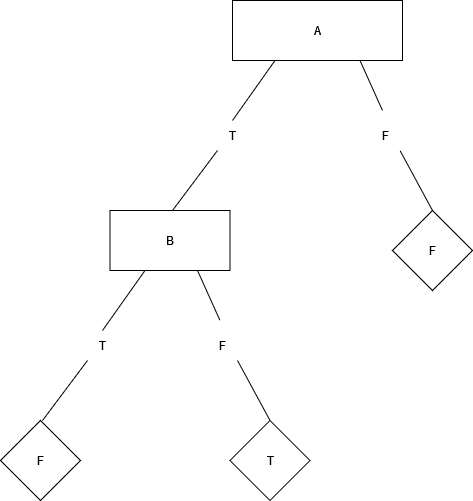
\includegraphics[width=120mm]{Untitled Diagram3.png} 
			\caption{a)}
		\end{figure}
	
	\newpage
	
	\paragraph{b)} $A \lor (B \land C)$
	\begin{figure}[H]
		\centering
		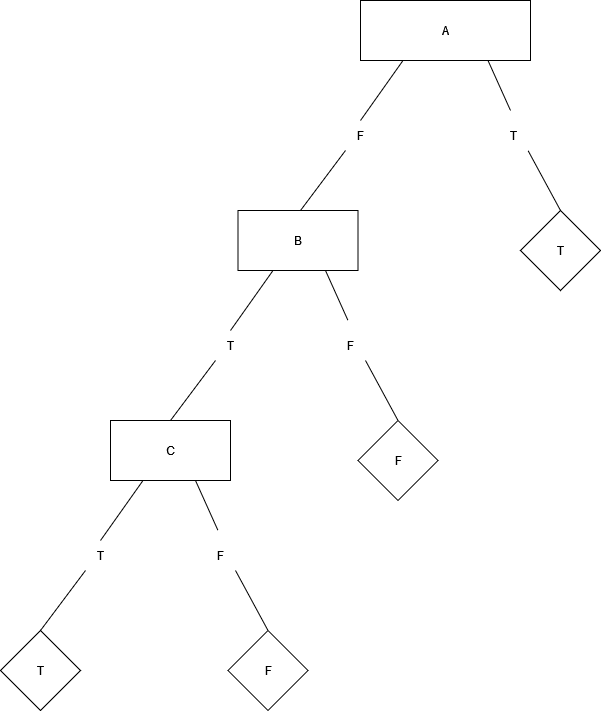
\includegraphics[width=120mm]{Untitled Diagram4.png} 
		\caption{b)}
	\end{figure}

	\newpage

	\paragraph{c)} $(A \land B) \lor (C \land D)$
	\begin{figure}[H]
		\centering
		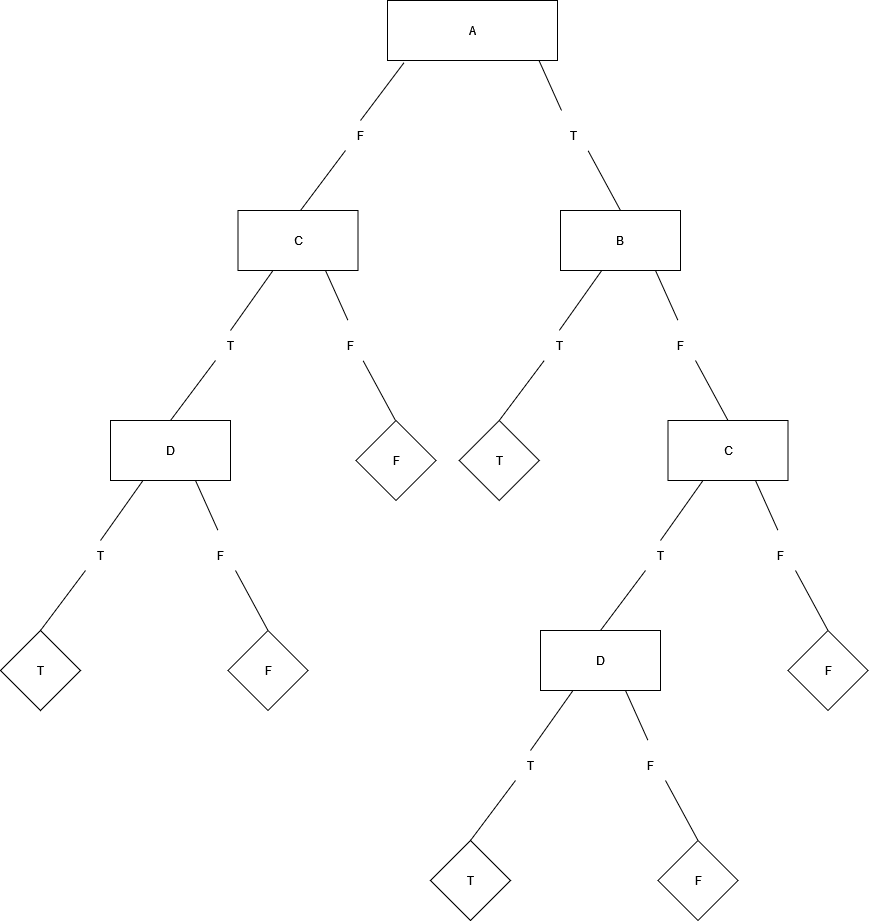
\includegraphics[width=150mm]{Untitled Diagram5.png} 
		\caption{c)}
	\end{figure}
	
	\newpage
	
	\section{Решение на задача \textnumero 4}
	
	Нека D1 и D2 са класификационни дървета описващи булеви функции (като тези от Задача \textnumero 3), такива че D2 е получено от D1 чрез заместване на листо (термален възел) в D1 с цяло поддърво T'.\newline
	\newline
	Ще покажем, че твърдението:
	\subparagraph{}
	\textit{D1 e \textbf{по-общо-или-равно-на} D2}
	\newline\newline
	е \textbf{не}винаги в сила.
	
	\paragraph{1)} Нека за простота D1 се описва чрез израза:
	\subparagraph{}
	$A$
	\subparagraph{}
	Тогава D1 ще изглежда така:
	
	\begin{figure}[H]
		\centering
		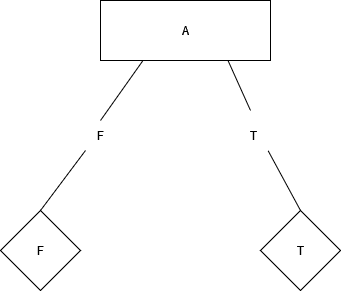
\includegraphics[width=60mm]{Untitled Diagram8.png} 
		\caption{D1}
	\end{figure}
	
	\paragraph{1)} Нека получим израз за D2 от този на D1 чрез добавяне на непразния (състоящ се поне от променлива B) израз на поддърво $T'$ посредством дизюнкция:
	\subparagraph{}
	$A \lor T'$
	\subparagraph{}
	Тогава D2 най-общо ще изглежда така:
	
	\begin{figure}[H]
		\centering
		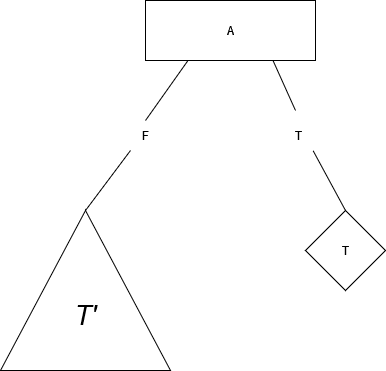
\includegraphics[width=80mm]{Untitled Diagram9.png} 
		\caption{D2}
	\end{figure}
	
	Забелязваме, че вече оценката на пример с $A = F$ не е директно F, а вече зависи от резултата от минаването по поддървото $T'$. Ако резултатът от това минаване е Т, тогава общия резултат ще е Т противно на резултатът F, получен при $A = F$ в D1. Tова би означавало противоречие с твърдението, тъй като примерът $A = F \land T' = T$ се покрива от хипотезата D2, но не от хипотезата D1. Нека за простота изразът описващ поддървото $T'$ е равен на B. Тоест израза за D2 става:
	\subparagraph{}
	$A \lor B$
	\newline\newline
	Тогава D2 ще изглежда по следния начин:
	\begin{figure}[H]
		\centering
		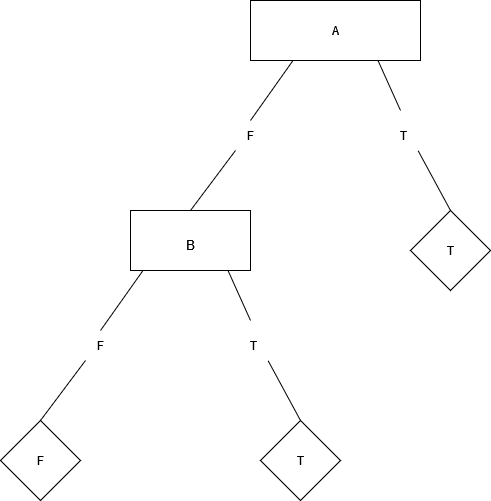
\includegraphics[width=80mm]{Untitled Diagram10.png} 
		\caption{D2}
	\end{figure}
	
	Нека разгледаме примерът $x \equiv A = F \land B = T$. Той се покрива от хипотезата D2 ($D2(x) = T$), но не се покрива от хипотезата D1 ($D1(x) = F$). D1 го ``изпуска''. Достигнахме до противоречие с твърдението \textit{D1 e \textbf{по-общо-или-равно-на} D2}. $\square$
	
\end{document}